% Options for packages loaded elsewhere
\PassOptionsToPackage{unicode}{hyperref}
\PassOptionsToPackage{hyphens}{url}
%
\documentclass[
  ignorenonframetext,
]{beamer}
\usepackage{pgfpages}
\setbeamertemplate{caption}[numbered]
\setbeamertemplate{caption label separator}{: }
\setbeamercolor{caption name}{fg=normal text.fg}
\beamertemplatenavigationsymbolsempty
% Prevent slide breaks in the middle of a paragraph
\widowpenalties 1 10000
\raggedbottom
\setbeamertemplate{part page}{
  \centering
  \begin{beamercolorbox}[sep=16pt,center]{part title}
    \usebeamerfont{part title}\insertpart\par
  \end{beamercolorbox}
}
\setbeamertemplate{section page}{
  \centering
  \begin{beamercolorbox}[sep=12pt,center]{part title}
    \usebeamerfont{section title}\insertsection\par
  \end{beamercolorbox}
}
\setbeamertemplate{subsection page}{
  \centering
  \begin{beamercolorbox}[sep=8pt,center]{part title}
    \usebeamerfont{subsection title}\insertsubsection\par
  \end{beamercolorbox}
}
\AtBeginPart{
  \frame{\partpage}
}
\AtBeginSection{
  \ifbibliography
  \else
    \frame{\sectionpage}
  \fi
}
\AtBeginSubsection{
  \frame{\subsectionpage}
}
\usepackage{lmodern}
\usepackage{amssymb,amsmath}
\usepackage{ifxetex,ifluatex}
\ifnum 0\ifxetex 1\fi\ifluatex 1\fi=0 % if pdftex
  \usepackage[T1]{fontenc}
  \usepackage[utf8]{inputenc}
  \usepackage{textcomp} % provide euro and other symbols
\else % if luatex or xetex
  \usepackage{unicode-math}
  \defaultfontfeatures{Scale=MatchLowercase}
  \defaultfontfeatures[\rmfamily]{Ligatures=TeX,Scale=1}
\fi
% Use upquote if available, for straight quotes in verbatim environments
\IfFileExists{upquote.sty}{\usepackage{upquote}}{}
\IfFileExists{microtype.sty}{% use microtype if available
  \usepackage[]{microtype}
  \UseMicrotypeSet[protrusion]{basicmath} % disable protrusion for tt fonts
}{}
\makeatletter
\@ifundefined{KOMAClassName}{% if non-KOMA class
  \IfFileExists{parskip.sty}{%
    \usepackage{parskip}
  }{% else
    \setlength{\parindent}{0pt}
    \setlength{\parskip}{6pt plus 2pt minus 1pt}}
}{% if KOMA class
  \KOMAoptions{parskip=half}}
\makeatother
\usepackage{xcolor}
\IfFileExists{xurl.sty}{\usepackage{xurl}}{} % add URL line breaks if available
\IfFileExists{bookmark.sty}{\usepackage{bookmark}}{\usepackage{hyperref}}
\hypersetup{
  pdftitle={Module 3: Pipeline and Deterministic ER},
  pdfauthor={Rebecca C. Steorts},
  hidelinks,
  pdfcreator={LaTeX via pandoc}}
\urlstyle{same} % disable monospaced font for URLs
\newif\ifbibliography
\usepackage{color}
\usepackage{fancyvrb}
\newcommand{\VerbBar}{|}
\newcommand{\VERB}{\Verb[commandchars=\\\{\}]}
\DefineVerbatimEnvironment{Highlighting}{Verbatim}{commandchars=\\\{\}}
% Add ',fontsize=\small' for more characters per line
\usepackage{framed}
\definecolor{shadecolor}{RGB}{248,248,248}
\newenvironment{Shaded}{\begin{snugshade}}{\end{snugshade}}
\newcommand{\AlertTok}[1]{\textcolor[rgb]{0.94,0.16,0.16}{#1}}
\newcommand{\AnnotationTok}[1]{\textcolor[rgb]{0.56,0.35,0.01}{\textbf{\textit{#1}}}}
\newcommand{\AttributeTok}[1]{\textcolor[rgb]{0.77,0.63,0.00}{#1}}
\newcommand{\BaseNTok}[1]{\textcolor[rgb]{0.00,0.00,0.81}{#1}}
\newcommand{\BuiltInTok}[1]{#1}
\newcommand{\CharTok}[1]{\textcolor[rgb]{0.31,0.60,0.02}{#1}}
\newcommand{\CommentTok}[1]{\textcolor[rgb]{0.56,0.35,0.01}{\textit{#1}}}
\newcommand{\CommentVarTok}[1]{\textcolor[rgb]{0.56,0.35,0.01}{\textbf{\textit{#1}}}}
\newcommand{\ConstantTok}[1]{\textcolor[rgb]{0.00,0.00,0.00}{#1}}
\newcommand{\ControlFlowTok}[1]{\textcolor[rgb]{0.13,0.29,0.53}{\textbf{#1}}}
\newcommand{\DataTypeTok}[1]{\textcolor[rgb]{0.13,0.29,0.53}{#1}}
\newcommand{\DecValTok}[1]{\textcolor[rgb]{0.00,0.00,0.81}{#1}}
\newcommand{\DocumentationTok}[1]{\textcolor[rgb]{0.56,0.35,0.01}{\textbf{\textit{#1}}}}
\newcommand{\ErrorTok}[1]{\textcolor[rgb]{0.64,0.00,0.00}{\textbf{#1}}}
\newcommand{\ExtensionTok}[1]{#1}
\newcommand{\FloatTok}[1]{\textcolor[rgb]{0.00,0.00,0.81}{#1}}
\newcommand{\FunctionTok}[1]{\textcolor[rgb]{0.00,0.00,0.00}{#1}}
\newcommand{\ImportTok}[1]{#1}
\newcommand{\InformationTok}[1]{\textcolor[rgb]{0.56,0.35,0.01}{\textbf{\textit{#1}}}}
\newcommand{\KeywordTok}[1]{\textcolor[rgb]{0.13,0.29,0.53}{\textbf{#1}}}
\newcommand{\NormalTok}[1]{#1}
\newcommand{\OperatorTok}[1]{\textcolor[rgb]{0.81,0.36,0.00}{\textbf{#1}}}
\newcommand{\OtherTok}[1]{\textcolor[rgb]{0.56,0.35,0.01}{#1}}
\newcommand{\PreprocessorTok}[1]{\textcolor[rgb]{0.56,0.35,0.01}{\textit{#1}}}
\newcommand{\RegionMarkerTok}[1]{#1}
\newcommand{\SpecialCharTok}[1]{\textcolor[rgb]{0.00,0.00,0.00}{#1}}
\newcommand{\SpecialStringTok}[1]{\textcolor[rgb]{0.31,0.60,0.02}{#1}}
\newcommand{\StringTok}[1]{\textcolor[rgb]{0.31,0.60,0.02}{#1}}
\newcommand{\VariableTok}[1]{\textcolor[rgb]{0.00,0.00,0.00}{#1}}
\newcommand{\VerbatimStringTok}[1]{\textcolor[rgb]{0.31,0.60,0.02}{#1}}
\newcommand{\WarningTok}[1]{\textcolor[rgb]{0.56,0.35,0.01}{\textbf{\textit{#1}}}}
\setlength{\emergencystretch}{3em} % prevent overfull lines
\providecommand{\tightlist}{%
  \setlength{\itemsep}{0pt}\setlength{\parskip}{0pt}}
\setcounter{secnumdepth}{-\maxdimen} % remove section numbering
% Custom definitions
% To use this customization file, insert the line "\input{custom}" in the header of the tex file.

% Formatting




% Packages

\setbeamertemplate{navigation symbols}{}
\setbeamertemplate{footline}[page number]

 \usepackage{amssymb,latexsym}
\usepackage{amssymb,amsfonts,amsmath,latexsym,amsthm, bm}
%\usepackage[usenames,dvipsnames]{color}
%\usepackage[]{graphicx}
%\usepackage[space]{grffile}
\usepackage{mathrsfs}   % fancy math font
% \usepackage[font=small,skip=0pt]{caption}
%\usepackage[skip=0pt]{caption}
%\usepackage{subcaption}
%\usepackage{verbatim}
%\usepackage{url}
%\usepackage{bm}
\usepackage{dsfont}
\usepackage{multirow}
%\usepackage{extarrows}
%\usepackage{multirow}
%% \usepackage{wrapfig}
%% \usepackage{epstopdf}
%\usepackage{rotating}
%\usepackage{tikz}
%\usetikzlibrary{fit}					% fitting shapes to coordinates
%\usetikzlibrary{backgrounds}	% drawing the background after the foreground


% \usepackage[dvipdfm,colorlinks,citecolor=blue,linkcolor=blue,urlcolor=blue]{hyperref}
%\usepackage[colorlinks,citecolor=blue,linkcolor=blue,urlcolor=blue]{hyperref}
%%\usepackage{hyperref}
%\usepackage[authoryear,round]{natbib}


%  Theorems, etc.

%\theoremstyle{plain}
%\newtheorem{theorem}{Theorem}[section]
%\newtheorem{corollary}[theorem]{Corollary}
%\newtheorem{lemma}[theorem]{Lemma}
%\newtheorem{proposition}[theorem]{Proposition}
%\newtheorem{condition}[theorem]{Condition}
% \newtheorem{conditions}[theorem]{Conditions}

%\theoremstyle{definition}
%\newtheorem{definition}[theorem]{Definition}
%% \newtheorem*{unnumbered-definition}{Definition}
%\newtheorem{example}[theorem]{Example}
%\theoremstyle{remark}
%\newtheorem*{remark}{Remark}
%\numberwithin{equation}{section}




% Document-specific shortcuts
\newcommand{\btheta}{{\bm\theta}}
\newcommand{\bbtheta}{{\pmb{\bm\theta}}}

\newcommand{\commentary}[1]{\ifx\showcommentary\undefined\else \emph{#1}\fi}

\newcommand{\term}[1]{\textit{\textbf{#1}}}

% Math shortcuts

% Probability distributions
\DeclareMathOperator*{\Exp}{Exp}
\DeclareMathOperator*{\TExp}{TExp}
\DeclareMathOperator*{\Bernoulli}{Bernoulli}
\DeclareMathOperator*{\Beta}{Beta}
\DeclareMathOperator*{\Ga}{Gamma}
\DeclareMathOperator*{\TGamma}{TGamma}
\DeclareMathOperator*{\Poisson}{Poisson}
\DeclareMathOperator*{\Binomial}{Binomial}
\DeclareMathOperator*{\NormalGamma}{NormalGamma}
\DeclareMathOperator*{\InvGamma}{InvGamma}
\DeclareMathOperator*{\Cauchy}{Cauchy}
\DeclareMathOperator*{\Uniform}{Uniform}
\DeclareMathOperator*{\Gumbel}{Gumbel}
\DeclareMathOperator*{\Pareto}{Pareto}
\DeclareMathOperator*{\Mono}{Mono}
\DeclareMathOperator*{\Geometric}{Geometric}
\DeclareMathOperator*{\Wishart}{Wishart}

% Math operators
\DeclareMathOperator*{\argmin}{arg\,min}
\DeclareMathOperator*{\argmax}{arg\,max}
\DeclareMathOperator*{\Cov}{Cov}
\DeclareMathOperator*{\diag}{diag}
\DeclareMathOperator*{\median}{median}
\DeclareMathOperator*{\Vol}{Vol}

% Math characters
\newcommand{\R}{\mathbb{R}}
\newcommand{\Z}{\mathbb{Z}}
\newcommand{\E}{\mathbb{E}}
\renewcommand{\Pr}{\mathbb{P}}
\newcommand{\I}{\mathds{1}}
\newcommand{\V}{\mathbb{V}}

\newcommand{\A}{\mathcal{A}}
%\newcommand{\C}{\mathcal{C}}
\newcommand{\D}{\mathcal{D}}
\newcommand{\Hcal}{\mathcal{H}}
\newcommand{\M}{\mathcal{M}}
\newcommand{\N}{\mathcal{N}}
\newcommand{\X}{\mathcal{X}}
\newcommand{\Zcal}{\mathcal{Z}}
\renewcommand{\P}{\mathcal{P}}

\newcommand{\T}{\mathtt{T}}
\renewcommand{\emptyset}{\varnothing}


% Miscellaneous commands
\newcommand{\iid}{\stackrel{\mathrm{iid}}{\sim}}
\newcommand{\matrixsmall}[1]{\bigl(\begin{smallmatrix}#1\end{smallmatrix} \bigr)}

\newcommand{\items}[1]{\begin{itemize} #1 \end{itemize}}

\newcommand{\todo}[1]{\emph{\textcolor{red}{(#1)}}}

\newcommand{\branch}[4]{
\left\{
	\begin{array}{ll}
		#1  & \mbox{if } #2 \\
		#3 & \mbox{if } #4
	\end{array}
\right.
}

% approximately proportional to
\def\app#1#2{%
  \mathrel{%
    \setbox0=\hbox{$#1\sim$}%
    \setbox2=\hbox{%
      \rlap{\hbox{$#1\propto$}}%
      \lower1.3\ht0\box0%
    }%
    \raise0.25\ht2\box2%
  }%
}
\def\approxprop{\mathpalette\app\relax}

% \newcommand{\approptoinn}[2]{\mathrel{\vcenter{
  % \offinterlineskip\halign{\hfil$##$\cr
    % #1\propto\cr\noalign{\kern2pt}#1\sim\cr\noalign{\kern-2pt}}}}}

% \newcommand{\approxpropto}{\mathpalette\approptoinn\relax}

\title{Module 3: Pipeline and Deterministic ER}
\author{Rebecca C. Steorts}
\date{}

\begin{document}
\frame{\titlepage}

\begin{frame}{Reading}
\protect\hypertarget{reading}{}

\begin{itemize}
\tightlist
\item
  Binette and Steorts (2020)
\item
  Christen (2012), Chapters 1-3
\end{itemize}

\end{frame}

\begin{frame}{Agenda}
\protect\hypertarget{agenda}{}

\begin{itemize}
\tightlist
\item
  Pipeline Approach
\item
  Deterministic Record Linkage
\item
  Exact Matching
\item
  Scoring Functions
\item
  Application to El Salvador
\end{itemize}

\end{frame}

\begin{frame}[fragile]{Load R packages}
\protect\hypertarget{load-r-packages}{}

\begin{Shaded}
\begin{Highlighting}[]
\KeywordTok{library}\NormalTok{(RecordLinkage)}
\end{Highlighting}
\end{Shaded}

\end{frame}

\begin{frame}{Data Cleaning Pipeline}
\protect\hypertarget{data-cleaning-pipeline}{}

\begin{figure}
  \begin{center}
    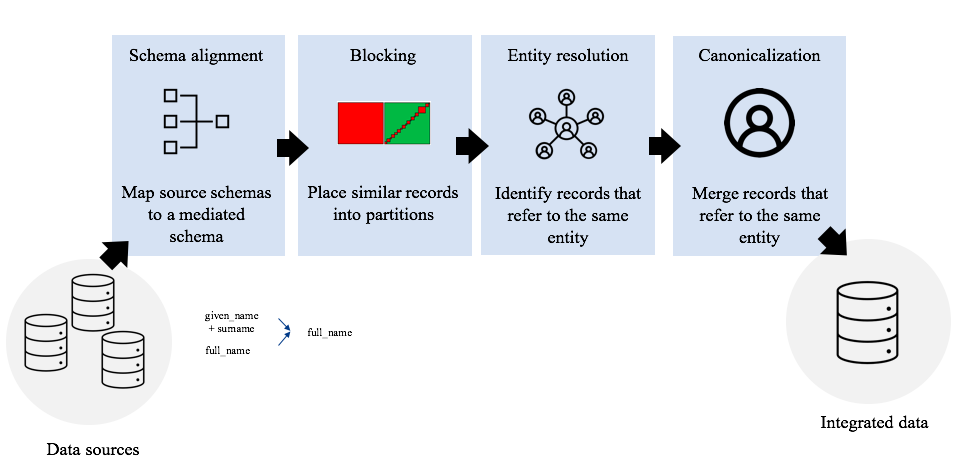
\includegraphics[width=\textwidth]{finalFigures/pipeline}
    \caption{Data cleaning pipeline.}
    \end{center}
\end{figure}

\end{frame}

\begin{frame}{Deterministic Record Linkage}
\protect\hypertarget{deterministic-record-linkage}{}

The most commonly used record linkage methods are based on a series of
deterministic rules involving the comparison of record attributes.

\end{frame}

\begin{frame}{Exact Matching and off by \(k\) matching}
\protect\hypertarget{exact-matching-and-off-by-k-matching}{}

\begin{itemize}
\tightlist
\item
  Exact matching is where two record pairs are linked if they agree on
  all common attributes.
\end{itemize}

\pause

\begin{itemize}
\tightlist
\item
  Off by one matching links records pairs if they link on all common
  attributes (except for one).
\end{itemize}

\pause

\begin{itemize}
\tightlist
\item
  Off by two matching links record pairs if they link on all common
  attributes (except for two).
\end{itemize}

\pause

\end{frame}

\begin{frame}{Exact Matching and off by \(k\) matching}
\protect\hypertarget{exact-matching-and-off-by-k-matching-1}{}

An extension, off by k-matching, states that two record pairs are a
match if they match on all common attributes except at most k, where k
is an integer larger than 0.

\vspace*{2em}

\pause

Exact matching (or extensions) are used when all the attributes are
categorical as it tends to perform well, as opposed to when textual
variables are introduced.

\end{frame}

\begin{frame}[fragile]{RLdata500}
\protect\hypertarget{rldata500}{}

Consider the \texttt{RLdata500} data set, removing any columns that
contain missing values.

\begin{Shaded}
\begin{Highlighting}[]
\KeywordTok{library}\NormalTok{(blink) }\CommentTok{# load RLdata500}
\KeywordTok{data}\NormalTok{(RLdata500)}
\NormalTok{data <-}\StringTok{ }\NormalTok{RLdata500[}\OperatorTok{-}\KeywordTok{c}\NormalTok{(}\DecValTok{2}\NormalTok{,}\DecValTok{4}\NormalTok{)] }\CommentTok{# Remove missing values}
\KeywordTok{head}\NormalTok{(data)}
\end{Highlighting}
\end{Shaded}

\begin{verbatim}
##   fname_c1 lname_c1   by bm bd
## 1  CARSTEN    MEIER 1949  7 22
## 2     GERD    BAUER 1968  7 27
## 3   ROBERT HARTMANN 1930  4 30
## 4   STEFAN    WOLFF 1957  9  2
## 5     RALF  KRUEGER 1966  1 13
## 6  JUERGEN   FRANKE 1929  7  4
\end{verbatim}

\end{frame}

\begin{frame}[fragile]{All pairs of records}
\protect\hypertarget{all-pairs-of-records}{}

Now let's consider all possible pairs of records.

\begin{Shaded}
\begin{Highlighting}[]
\CommentTok{# create all pairs of records}
\NormalTok{pairs <-}\StringTok{ }\KeywordTok{t}\NormalTok{(}\KeywordTok{combn}\NormalTok{(}\DecValTok{1}\OperatorTok{:}\KeywordTok{nrow}\NormalTok{(RLdata500), }\DecValTok{2}\NormalTok{))}
\KeywordTok{head}\NormalTok{(pairs)}
\end{Highlighting}
\end{Shaded}

\begin{verbatim}
##      [,1] [,2]
## [1,]    1    2
## [2,]    1    3
## [3,]    1    4
## [4,]    1    5
## [5,]    1    6
## [6,]    1    7
\end{verbatim}

\end{frame}

\begin{frame}[fragile]{Pairwise features that disagree}
\protect\hypertarget{pairwise-features-that-disagree}{}

For each pair of records, compute the number of features that
disagree.\footnote{This takes a few minute to compute in \texttt{R}. (There are more efficient ways to do this).}

\begin{Shaded}
\begin{Highlighting}[]
\NormalTok{n_disagree =}\StringTok{ }\KeywordTok{sapply}\NormalTok{(}\DecValTok{1}\OperatorTok{:}\KeywordTok{nrow}\NormalTok{(pairs), }\ControlFlowTok{function}\NormalTok{(i) \{}
\NormalTok{  recordA =}\StringTok{ }\NormalTok{data[pairs[i,}\DecValTok{1}\NormalTok{],]}
\NormalTok{  recordB =}\StringTok{ }\NormalTok{data[pairs[i,}\DecValTok{2}\NormalTok{],]}
  \KeywordTok{sum}\NormalTok{(recordA }\OperatorTok{!=}\StringTok{ }\NormalTok{recordB)}
\NormalTok{\})}
\end{Highlighting}
\end{Shaded}

\end{frame}

\begin{frame}[fragile]{Distribution of Feature Disagreement Among Record
Pairs}
\protect\hypertarget{distribution-of-feature-disagreement-among-record-pairs}{}

\footnotesize

\begin{Shaded}
\begin{Highlighting}[]
\KeywordTok{plot}\NormalTok{(}\KeywordTok{table}\NormalTok{(n_disagree), }
     \DataTypeTok{xlab=}\StringTok{"Number of features that  disagree"}\NormalTok{,}
     \DataTypeTok{ylab=}\StringTok{"Total number of record pairs"}\NormalTok{)}
\end{Highlighting}
\end{Shaded}

\begin{center}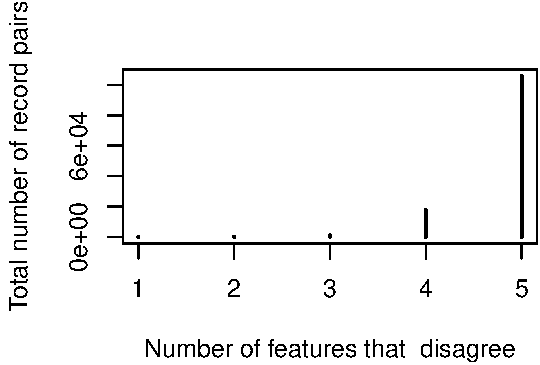
\includegraphics{pipeline-approaches_files/figure-beamer/unnamed-chunk-5-1} \end{center}

\end{frame}

\begin{frame}{What do you observe?}
\protect\hypertarget{what-do-you-observe}{}

\footnotesize

\begin{center}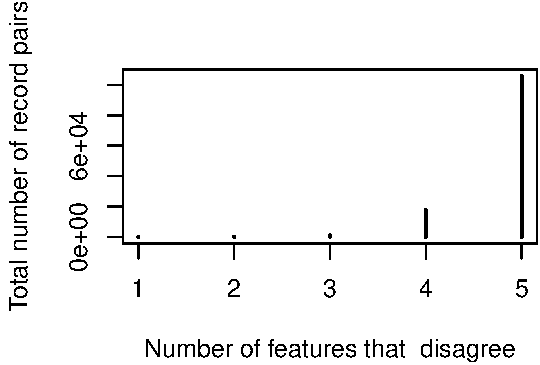
\includegraphics{pipeline-approaches_files/figure-beamer/unnamed-chunk-6-1} \end{center}

\end{frame}

\begin{frame}{Distribution of Feature Disagreement Among Record Pairs}
\protect\hypertarget{distribution-of-feature-disagreement-among-record-pairs-1}{}

\begin{itemize}
\tightlist
\item
  Observe that record pairs disagree on four or 5 features. We expect
  these records to not be matched.
\end{itemize}

\pause

\begin{itemize}
\tightlist
\item
  Pairs disagreeing only on 1, 2 or 3 features \emph{might} be matches.
\end{itemize}

\pause

\vspace*{2em}

Is this intuitive?

\end{frame}

\begin{frame}{Exact Matching, Etc}
\protect\hypertarget{exact-matching-etc}{}

Now, let's investigate exact matching (and extensions) on the
\texttt{RLdata500} data set.

\end{frame}

\begin{frame}[fragile]{Exact Matching}
\protect\hypertarget{exact-matching}{}

\textbf{Exact matching:} Link record pairs that agree on all features.

\vspace*{1em}

\begin{Shaded}
\begin{Highlighting}[]
\KeywordTok{sum}\NormalTok{(n_disagree }\OperatorTok{==}\StringTok{ }\DecValTok{0}\NormalTok{)}
\end{Highlighting}
\end{Shaded}

\begin{verbatim}
## [1] 0
\end{verbatim}

\vspace*{1em}

No pairs are exact matches!

\end{frame}

\begin{frame}[fragile]{Off by one matching}
\protect\hypertarget{off-by-one-matching}{}

\textbf{Off by 1 matching:} Link record pairs that disagree only in one
feature.

\vspace*{1em}
\footnotesize

\begin{Shaded}
\begin{Highlighting}[]
\CommentTok{# Links}
\NormalTok{links =}\StringTok{ }\NormalTok{pairs[n_disagree }\OperatorTok{<=}\StringTok{ }\DecValTok{1}\NormalTok{, ]}

\CommentTok{# Number of estimated links}
\KeywordTok{nrow}\NormalTok{(links)}
\end{Highlighting}
\end{Shaded}

\begin{verbatim}
## [1] 46
\end{verbatim}

\begin{Shaded}
\begin{Highlighting}[]
\CommentTok{# Number of correctly estimated links}
\KeywordTok{sum}\NormalTok{(}\KeywordTok{sapply}\NormalTok{(}\DecValTok{1}\OperatorTok{:}\KeywordTok{nrow}\NormalTok{(links), }\ControlFlowTok{function}\NormalTok{(i) \{}
\NormalTok{  identity.RLdata500[links[i,}\DecValTok{1}\NormalTok{]] }\OperatorTok{==}\StringTok{ }
\StringTok{    }\NormalTok{identity.RLdata500[links[i,}\DecValTok{2}\NormalTok{]]}
\NormalTok{\}))}
\end{Highlighting}
\end{Shaded}

\begin{verbatim}
## [1] 46
\end{verbatim}

\end{frame}

\begin{frame}{Off by two matching}
\protect\hypertarget{off-by-two-matching}{}

How would you extend this to off by two matching?

What do you find?

\end{frame}

\begin{frame}{Scoring Rules}
\protect\hypertarget{scoring-rules}{}

We now turn to scoring rules and how these are used in entity resolution
tasks.

\end{frame}

\begin{frame}{Scoring Rules}
\protect\hypertarget{scoring-rules-1}{}

\begin{itemize}
\item
  Record attributes are often distorted by noise. Why would this occur?
\item
  Linkage rules should account for such noise, distortions, and errors
  through scoring rules or functions.
\item
  Examples commonly used for westernized names are the Edit
  (Levenshtein), Jaro, and Jaro-Winkler distance functions.
\end{itemize}

\end{frame}

\begin{frame}{Edit (Levenshtein) distance (1966)}
\protect\hypertarget{edit-levenshtein-distance-1966}{}

The Edit distance calculates the minimum number of substitutions
required to transform a string \(s_1\) into a string \(s_2.\)

Formally, \[\text{Edit} = 1-\frac{L}{maxLength(s_1, s_2)}.\]

\end{frame}

\begin{frame}{Example}
\protect\hypertarget{example}{}

Consider the number of substitutions required to transform from
\textbf{Adam} to \textbf{Alan.} Use the Edit distance formulate to find
the similarity score that is between \([0,1].\)

\end{frame}

\begin{frame}{Solution}
\protect\hypertarget{solution}{}

The number of substitutions required is \(L=2.\)

This is normalized into a similarity function using the following:

\[\text{Edit} = 1-\frac{L}{maxLength(s_1, s_2)} = 1-2/4=1-0.5=0.5\]

\end{frame}

\begin{frame}[fragile]{Solution}
\protect\hypertarget{solution-1}{}

Let's verify this in \texttt{R}.

\begin{Shaded}
\begin{Highlighting}[]
\NormalTok{s1 <-}\StringTok{ "Adam"}
\NormalTok{s2 <-}\StringTok{ "Alan"}
\KeywordTok{levenshteinSim}\NormalTok{(}\StringTok{"s1"}\NormalTok{, }\StringTok{"s2"}\NormalTok{)}
\end{Highlighting}
\end{Shaded}

\begin{verbatim}
## [1] 0.5
\end{verbatim}

\end{frame}

\begin{frame}{Jaro-Winkler}
\protect\hypertarget{jaro-winkler}{}

\begin{itemize}
\item
  The Jaro distance (1989), called J, considered common characters and
  character transpositions.
\item
  The Jaro-Winkler (1990) similarity measure, denoted JW is:
\end{itemize}

\begin{center}
$ JW(A,B)= J(A,B) + \textcolor{red}{0.1p}(1-J(A,B)) $
\end{center}

where \(p\) is the \# of the first four characters that agree exactly.

\end{frame}

\begin{frame}{Example}
\protect\hypertarget{example-1}{}

Let's return to the example of comparing Adam and Alan.

\begin{itemize}
\item
  Here, \(p = 1.\)
\item
  Given the complexity, we will calculate J and JW using \texttt{R}.
\end{itemize}

\end{frame}

\begin{frame}[fragile]{Example}
\protect\hypertarget{example-2}{}

\begin{Shaded}
\begin{Highlighting}[]
\CommentTok{## It seems Jaro is not supported in R}
\KeywordTok{jarowinkler}\NormalTok{(s1,s2)}
\end{Highlighting}
\end{Shaded}

\begin{verbatim}
## [1] 0.7
\end{verbatim}

e.g.~Adam vs Alan: p=1, J= 0.67 and JW=0.7.

These work well on English names that are less than 7 characters.

\end{frame}

\begin{frame}{Other distance functions}
\protect\hypertarget{other-distance-functions}{}

There are many other distance functions, such as the Jaccard, Hamming,
and Cosine distances just to name a few.

\end{frame}

\begin{frame}{Recap}
\protect\hypertarget{recap}{}

You should now be familiar with the following:

\begin{itemize}
\tightlist
\item
  the pipeline approach
\item
  deterministic record linkage methods
\item
  exact matching and extensions
\item
  scoring functions
\end{itemize}

Discussion: How might you put these rules together to form more complex
entity resolution rules?

\end{frame}

\end{document}
